% vim: textwidth=80
\documentclass{llncs}
%\usepackage{fullpage}

%\usepackage[utf8]{inputenc}
\usepackage{amsmath}
%\usepackage{amsthm}
\usepackage{graphicx}
\usepackage{caption}
\usepackage{subcaption}
\usepackage{amssymb}
\usepackage{amsfonts}
\usepackage{floatrow}

\title{On Coloring Resilient Graphs}
\author{Jeremy Kun \and Lev Reyzin}
\institute{
Department of Mathematics, Statistics, and Computer Science\\
University of Illinois at Chicago\\
Chicago, IL 60607\\
\texttt{\{jkun2,lreyzin\}@math.uic.edu}
}

\newtheorem{thm}{Theorem}
\newtheorem{cor}{Corollary}
\newtheorem{defn}{Definition}
\newtheorem{propn}{Proposition}
\newtheorem{obs}{Observation}
\newtheorem{prob}{Problem}


\date{}


\begin{document}
\maketitle

\begin{abstract} 
We introduce a new notion of resilience for constraint satisfaction problems,
with the goal of more precisely determining the boundary between NP-hardness
and the existence of efficient algorithms for resilient instances.  In
particular, we study $r$-resiliently $k$-colorable graphs, which are those
$k$-colorable graphs that remain $k$-colorable even after the addition of any
$r$ new edges.  We prove lower bounds on the NP-hardness of coloring
resiliently colorable graphs, and provide an algorithm that colors sufficiently
resilient graphs. This notion of resilience suggests an array of open
questions for graph colorability and other combinatorial problems.
\end{abstract}

\section{Introduction and related work}

An important goal in studying NP-complete combinatorial problems is to find
precise boundaries between tractability and NP-hardness. This is often done by
adding constraints to the instances being considered until a polynomial time
algorithm is found.  For instance, while SAT is NP-hard, the restricted $2$-SAT
and XOR-SAT versions are decidable in polynomial time.  

In this paper we present a new angle for studying the boundary between NP-hardness
and tractability.
We informally define the resilience of a constraint-based combinatorial problem
and we focus on the case of resilient graph colorability. Roughly speaking, a
positive instance is resilient if it remains a positive instance up to the
addition of a constraint. For example, an instance $G$ of Hamiltonian circuit
would be ``$r$-resilient'' if $G$ has a Hamiltonian circuit, and $G$ minus any
$r$ edges \emph{still} has a Hamiltonian circuit. In the case of coloring, we
say a graph $G$ is $r$-resiliently $k$-colorable if $G$ is $k$-colorable and
will remain so even if any $r$ edges are added. One would imagine that
\emph{finding} an $r$-coloring in a very resilient graph would be easy, as that
instance is very ``far'' from being not colorable.  And in general, one can
pose the question: how resilient can instances be and have the search problem
still remain hard?\footnote{We focus on the search versions of the problems
because the decision version on resilient instances induces the trivial ``yes''
answer.}

Most NP-hard problems have natural definitions of resiliency.  For instance,
resilient positive instances for optimization problems over graphs can be
defined as those that remain positive instances even up to the addition or
removal of any edge.  For satisfiability, we say a resilient instance is one
where variables can be ``fixed'' and the formula remains satisfiable. In
problems like set-cover, we could allow for the removal of a given number of
sets. Indeed, this can be seen as a general notion of resilience for adding
constraints in constraint satisfaction problems (CSPs), which have an extensive
literature~\cite{Kumar92}. However, a resilience definition for general CSPs
is not immediate because the ability to add any constraint (e.g., the negation
of an existing constraint) is too strong.

Therefore we focus on a specific combinatorial problem, graph coloring.
Resilience is defined up to the addition of edges, and we first show that this
is an interesting notion: many famous, well studied graphs exhibit strong
resilience properties. Then, perhaps surprisingly, we prove that $3$-coloring a
$1$-resiliently 3-colorable graph is NP-hard -- that is, it is hard to color a
graph even when it is guaranteed to remain $3$-colorable under the addition of
any edge. Briefly, our reduction works by mapping positive instances of 3-SAT
to 1-resiliently 3-colorable graphs and negative instances to graphs of
chromatic number at least 4. An algorithm which can color 1-resiliently
3-colorable graphs can hence distinguish between the two. On the other hand, we
observe that $3$-resiliently $3$-colorable graphs have polynomial-time coloring
algorithms (leaving the case of 3-coloring $2$-resiliently $3$-colorable graphs
tantalizingly open). We also show that efficient algorithms exist for
$k$-coloring $\binom{k}{2}$-resiliently $k$-colorable graphs for all $k$, and
discuss the implications of our lower bounds. 

This paper is organized as follows. In the next two subsections we review the
literature on other notions of resilience and on graph coloring. In
Section~\ref{sec:resilient-sat} we inspect a resilient version of 6-SAT which
lays the groundwork for our main theorem on 1-resilient 3-coloring. In
Section~\ref{sec:resilient-coloring-obs-bounds} we formally define the resilient
graph coloring problem and present preliminary upper and lower bounds. In
Section~\ref{sec:main-thm} we prove our main theorem, and in
Section~\ref{sec:open-problems} we discuss open problems.



\subsection{Related work on resilience}

There are related concepts of resilience in the literature. Perhaps the closest
in spirit is Bilu and Linial's notion of stability~\cite{BL12}.  Their notion
is restricted to problems over metric spaces and attempts to explain why
real-world instances are easy.  They argue that practical instances often
exhibit some degree of stability, which can make the problem easier.  Their
results on clustering stable instances have seen considerable interest and have
been substantially extended and improved~\cite{ABS10,BL12,Rey11}.  Their study
is also not limited to clustering -- for instance one can study TSP and other
optimization problems over metrics under the Bilu-Linial
assumption~\cite{MSSW11}.  
A related notion of stability by 
Ackerman and Ben-David~\cite{AckermanB09} for clustering 
yields efficient algorithms when the data lies in Euclidian space.

Our notion of resilience, on the other hand, is most natural in the case when
the optimization problem has natural constraints, which can be fixed or
modified.  Our primary goal is also different -- we seek to more finely
delineate the boundary between tractability and hardness in a systematic way
across problems.

Property testing can also be viewed as involving resilience. Roughly speaking
property testers are randomized algorithms which distinguish between
combinatorial structures that satisfy a property or are very far from satisfying
it. These algorithms are typically given access to a small sample depending on
$\varepsilon$ alone (and not the size of the input). For graph property testing,
as with resilience, the concept of being ``far'' from having a property involves
requiring the addition or removal of an arbitrary set of at most $\varepsilon
\binom{n}{2}$ edges from $G$. Our notion of resilience is different in that we
consider adding or removing a constant number of constraints. More importantly,
property testing is more concerned with query complexity than with
computational hardness, whereas we seek to relate the
complexity of search problems across varying degrees of resilience. 

\subsection{Previous work on coloring}

As the technical results of this paper are on graph colorability, we review
the relevant work.

A graph $G$ is $k$-colorable if there is an assignment of $k$ distinct colors
to the vertices of $G$ so that no edge is monochromatic. Determining whether
$G$ is $k$-colorable is a classic an NP-hard problem~\cite{Karp72}. Many 
attempts to simplify the problem, such as assuming planarity or bounded degree
of the graph in question, still result in NP-hardness~\cite{Dailey80}. A large
body of work surrounds positive and negative results for explicit families of
graphs. The list of families that are polynomial-time colorable includes
triangle-free planar graphs, perfect graphs and almost-perfect graphs, bounded
tree- and clique-width graphs, quadtrees, and various families of graphs
defined by the lack of an induced
subgraph~\cite{HMM10,Ko03,EBH99,Cai03,KKTW01}.

With little progress on coloring general graphs, research has naturally turned
to approximation. In approximating the chromatic number of a general graph, the
first results were of Garey and Johnson, giving a performance guarantee of
$O(n/\log n)$ colors~\cite{Johnson74} and proving that it is NP-hard to
approximate chromatic number to within a constant factor less than
two~\cite{GJ76}. Further work improved this bound by logarithmic factors
\cite{BR90,Ha93}. In terms of lower bounds, Zuckerman~\cite{Zu07} derandomized
the PCP-based results of H{\aa}stad~\cite{Ha99} to prove the best known
approximability lower-bound to date, $O(n^{1-\varepsilon})$.

There has been much recent interest in coloring graphs which are already known
to be colorable while minimizing the number of colors used. For a 3-colorable
graph, Widgerson gave an algorithm using at most $O(n^{1/2})$
colors~\cite{Wi83}, which Blum improved to $\tilde{O}(n^{3/8})$~\cite{Blum94}.
A line of research based on semidefinite programming and other combinatorial
improvements improved this bound still further to $\tilde{O}(n^{0.2072})$
\cite{Ka98,Blum97,Arora06,Chl09,KT12}. Despite the difficulties in improving
the constant in the exponent, and as suggested by Arora~\cite{Arora11}, there
is no evidence that coloring a 3-colorable graph with as few as $O(\log n)$
colors is hard.

On the other hand there are asymptotic and concrete lower bounds.
Khot~\cite{Khot01} proved that for sufficiently large $k$ it is NP-hard to
color a $k$-colorable graph with fewer than $k^{O(\log{k})}$ colors, and this
was recently improved by Huang to $2^{\sqrt[3]{k}}$~\cite{Huang13}. It is also
known that for every constant $h$ there exists a sufficiently large $k$ such
that coloring a $k$-colorable graph with $hk$ colors is NP-hard~\cite{DMR06}.
In the non-asymptotic case, Khanna, Linial, and Safra~\cite{KLS00} used the PCP
theorem to prove it is NP-hard to 4-color a 3-colorable graph, and more
generally to color a $k$ colorable graph with at most $k + 2\left \lfloor k/3
\right \rfloor - 1$ colors. Guruswami and Khanna later gave an explicit
reduction for $k=3$~\cite{GuKh2000}. Assuming a variant of Khot's 2-to-1
conjecture, Dinur et al. prove that distinguishing between chromatic number $K$
and $K'$ is hard for $3 \leq K < K'$~\cite{DMR06}.  Interestingly, this is the
best conditional lower bound we give in Section~\ref{sec:easy-bounds}, but it
does not to our knowledge imply Theorem~\ref{thm:3-1}.

Without large strides in approximate graph coloring, we need a new avenue to
approach the boundary between when coloring is difficult and when it is easy.
In this paper we consider the coloring problem for a general family of graphs
which we call \emph{resiliently colorable}, in the sense that adding edges does
not violate the given colorability assumption. 


\section{Warm up: resilient SAT}\label{sec:resilient-sat}

We begin by describing a resilient version of $k$-satisfiability, which is used
in proving our main result for resilient coloring in
Section~\ref{sec:main-thm}. 

\begin{prob}[resilient $k$-SAT]
A boolean formula $\varphi$ is \emph{$r$-resilient} if it is satisfiable
and remains satisfiable if any set of $r$ variables are fixed. We call
\emph{$r$-resilient $k$-SAT} the problem of finding a satisfying assignment for
an $r$-resiliently satisfiable $k$-CNF formula. Likewise, $r$-resilient CNF-SAT
is for $r$-resilient formulas in general CNF form.  
\end{prob}

While it is unclear exactly which values of $k$ and $r$ make this problem
NP-hard, the following proposition is straightforward. We use it in
Section~\ref{sec:main-thm} as the starting point for our main reduction. 

\begin{propn}
1-resilient 6-SAT is NP-hard.
\end{propn}
\begin{proof}
We reduce from 3-SAT. Let $\mathbf{x} = (x_1, \dots, x_n)$ and suppose
$\varphi(\mathbf{x})$ is an instance of 3-SAT.  Construct $\psi =
\varphi(\mathbf{x}) \vee \varphi(\mathbf{y})$ for some choice of new variables
$\mathbf{y} = (y_1, \dots, y_n)$, and put $\psi$ into 6-CNF form (which can be done in $O(n^2)$
steps). The formula $\varphi$ is satisfiable if and only if $\psi$ is, and
$\psi$ is 1-resilient: if any of the $x_i$ are fixed, we may satisfy $\varphi$
using the $y_i$ and vice versa if any of the $y_i$ are fixed.  
\end{proof}

\begin{cor}
For all fixed $r \geq 0$, $r$-resilient CNF-SAT is NP-hard.
\end{cor}
\begin{proof}
The previous proof can be modified to take a disjunction of $r+1$ copies of
$\varphi$, each with different variables. Call this new formula $\psi$.
Again $\varphi$ is satisfiable if and only if $\psi$ is, and we can put $\psi$
into CNF form in polynomial time. By the pigeonhole principle if $r$ variables
are fixed then at least one disjunct has all of its variables untouched, and we
can use this set of variables to satisfy $\psi$.  \end{proof}

\section{Resilient graph coloring and preliminary bounds}
\label{sec:resilient-coloring-obs-bounds}
\subsection{Problem definition and remarks}

\begin{prob}[resilient coloring] 
A graph $G$ is called \emph{$r$-resiliently $k$-colorable} if $G$ remains
$k$-colorable under the addition of any set of $r$ new edges.
\end{prob}

We argue that this notion is not trivial by showing the resilience properties
of some classic graphs. These were determined by exhaustive computer search.
%, and are displayed in Figure~\ref{fig:famous-graphs}.  
The Petersen graph is 2-resiliently 3-colorable. The D{\"u}rer graph is
1-resiliently 3-colorable (but not 2-resilient) and 4-resiliently 4-colorable
(but not 5-resilient). The Gr{\"o}tzsch graph is 4-resiliently 4-colorable (but
not 5-resilient). The Chv{\'a}tal graph is 3-resiliently 4-colorable (but not
4-resilient).

%\begin{figure}
%\centering
%\scalebox{0.45}{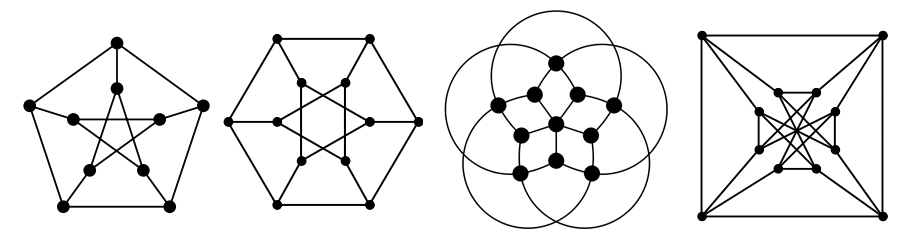
\includegraphics{famous-graphs.png}}
%\caption{From left to right: the Petersen graph, 2-resiliently 3-colorable;
%the D{\"u}rer graph, 4-resiliently 4-colorable; the Gr{\"o}tzsch graph,
%4-resiliently 4-colorable; and the Chv{\'a}tal graph, 3-resiliently
%4-colorable.} 
%\label{fig:famous-graphs}
%\end{figure}

There are a few interesting constructions to build intuition about resilient
graphs. First, it is clear that every $k$-colorable graph is 1-resiliently
$(k+1)$-colorable (just add one new color for the additional edge), but for all
$k > 2$ there exist $k$-colorable graphs which are not 2-resiliently
$(k+1)$-colorable. Simply remove two disjoint edges from the complete graph on
$k+2$ vertices. A slight generalization of this argument provides examples of
graphs which are $\left \lfloor (k+1)/2\right \rfloor$-colorable but not $\left
\lfloor (k+1)/2 \right \rfloor$-resiliently $k$-colorable for $k \geq 3$.
On the other hand, every $\left \lfloor (k+1)/2\right \rfloor$-colorable graph
is $(\left \lfloor (k+1)/2 \right \rfloor-1)$-resiliently $k$-colorable, since
$r$-resiliently $k$-colorable graphs are $(r+m)$-resiliently $(k+m)$-colorable
for all $m \geq 0$ (add one new color for each added edge). 

One expects high resilience in a $k$-colorable graph to reduce the number of
colors required to color it. While this may be true for super-linear
resilience, there are easy examples of $(k-1)$-resiliently $k$-colorable graphs
which are $k$-chromatic. For instance, add an isolated vertex to the complete
graph on $k$ vertices. The famous graphs above are also nice examples.

\subsection{Observations}

We are primarily interested in the complexity of coloring resilient graphs, and
so we pose the question: for which values of $k,r$ does the task of
$k$-coloring an $r$-resiliently $k$-colorable graph admit an efficient
algorithm? The following observations aid us in classifying such pairs. Using
these observations and the propositions in the following section, we fill in
the known complexities (including Theorem~\ref{thm:3-1}) in
Figure~\ref{fig:classification}.

\begin{obs}\label{obs:horizontal}
An $r$-resiliently $k$-colorable graph is $r'$-resiliently $k$-colorable for
any $r' \leq r$. Hence, if $k$-coloring is in P for $r$-resiliently
$k$-colorable graphs, then it is for $s$-resiliently $k$-colorable graphs for
all $s \geq r$.  Conversely, if $k$-coloring is NP-hard for $r$-resiliently
$k$-colorable graphs, then it is for $s$-resiliently $k$-colorable graphs for
all $s \leq r$. 
\end{obs}

This observation manifests itself in Figure~\ref{fig:classification} by the rule
that if a cell is in P, so are all of the cells to its right; and if a
cell is NP-hard, so are all of the cells to its left. 

\begin{obs}\label{obs:vertical}
If $k$-coloring is in P for $r$-resiliently $k$-colorable graphs, then
$k'$-coloring $r$-resiliently $k'$-colorable graphs is in P for all $k' \leq
k$. Similarly, if $k$-coloring is in NP-hard for $r$-resiliently $k$-colorable
graphs, then $k'$-coloring is NP-hard for $r$-resiliently $k'$-colorable graphs
for all $k' \geq k$.
\end{obs}
\begin{proof}
If $G$ is $r$-resiliently $k$-colorable, then we construct $G'$ by adding a
new vertex $v$ with complete incidence to $G$. Then $G'$ is $r$-resiliently
$(k+1)$-colorable, and an algorithm to color $G'$ can be used to color $G$.
\end{proof}

Observation~\ref{obs:vertical} yields the rule that if a cell is in P, so are
all of the cells above it; if a cell is NP-hard, so are the cells below it.
More generally, we have the following observation which allows us to apply
known bounds.

\begin{obs}\label{obs:function-bound}
If it is NP-hard to $f(k)$-color a $k$-colorable graph, then it is NP-hard to
$f(k)$-color an $(f(k)-k)$-resiliently $f(k)$-colorable graph.
\end{obs}

This observation is used in Propositions~\ref{propn:4-1}
and~\ref{propn:2-to-1-diagonal}, and follows from the fact that an
$r$-resiliently $k$-colorable graph is $(r+m)$-resiliently $(k+m)$-colorable
for all $m \geq 0$ (here $r = 0, m = f(k) - k$). 

\begin{figure}
\centering
\begin{subfigure}{.65\textwidth}
  \centering
  \scalebox{0.42}{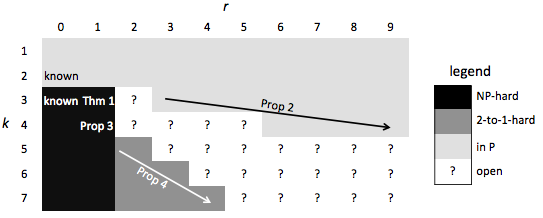
\includegraphics{table.png}}
\end{subfigure}%
\begin{subfigure}{.35\textwidth}
  \centering
  \scalebox{0.30}{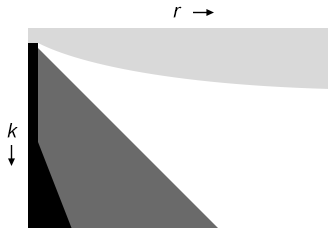
\includegraphics{zoomed-out.png}}
\end{subfigure}
\caption{The known classification of the complexity of $k$-coloring
$r$-resiliently $k$-colorable graphs. Left: the explicit classification for
small $k, r$. Right: a zoomed-out view of the same table, with the additional
NP-hard (black) region added by Proposition~\ref{propn:asymptotic}.}
\label{fig:classification} \end{figure}

\subsection{Upper and lower bounds} \label{sec:easy-bounds}
In this section we provide a simple upper bound on the complexity of coloring
resilient graphs, we apply known results to show that 4-coloring a
1-resiliently 4-colorable graph is NP-hard, and we give the conditional hardness
of $k$-coloring $(k-3)$-resiliently $k$-colorable graphs for all $k \geq 3$.
This last result follows from the work of Dinur et al., and depends a variant
of Khot's 2-to-1 conjecture~\cite{DMR06}. Finally, applying the result of
Huang~\cite{Huang13}, we give an unconditional asymptotic lower bound. These
results, along with our main theorem, are displayed graphically in
Figure~\ref{fig:classification}.

To explain Figure~\ref{fig:classification} more explicitly,
Proposition~\ref{propn:k-choose-2-bound} gives an upper bound for $r=
\binom{k}{2}$, and Proposition~\ref{propn:4-1} gives hardness of the cell $(4,1)$
and its consequences. Proposition~\ref{propn:2-to-1-diagonal} provides the
conditional lower bound, and Theorem~\ref{thm:3-1} gives the hardness of the cell
$(3,1)$. Finally, Proposition~\ref{propn:asymptotic} provides the asymptotic
lower bound.

\begin{propn}\label{propn:k-choose-2-bound}
There is an efficient algorithm for $k$-coloring $\binom{k}{2}$-resiliently
$k$-colorable graphs.
\end{propn}
\begin{proof}
If $G$ is $\binom{k}{2}$-resiliently $k$-colorable, then no vertex may have
degree $ \geq k$. For if $v$ is such a vertex, one may add complete incidence to
any choice of $k$ vertices in the neighborhood of $v$ to get $K_{k+1}$. Finally,
graphs with bounded degree $k-1$ are greedily $k$-colorable. 
\end{proof}

\begin{propn}\label{propn:4-1}
The problem of 4-coloring a 1-resiliently 4-colorable graph is NP-hard.
\end{propn}
\begin{proof}
It is known that 4-coloring a 3-colorable graph is NP-hard, so we may apply
Observation~\ref{obs:function-bound}. Every 3-colorable graph $G$ is
1-resiliently 4-colorable, since if we are given a proper 3-coloring of $G$ we
may use the fourth color to properly color any new edge that is added. So an
algorithm $A$ which efficiently 4-colors 1-resiliently 4-colorable graphs can be
used to 4-color a 3-colorable graph.
\end{proof}

We call a problem \emph{2-to-1-hard} if it is NP-hard under the condition that
Khot's 2-to-1 conjecture holds.

\begin{propn}\label{propn:2-to-1-diagonal}
For all $k \geq 3$, it is 2-to-1-hard to $k$-color a $(k-3)$-resiliently
$k$-colorable graph. 
\end{propn}
\begin{proof}
As with Proposition~\ref{propn:4-1}, we apply Observation~\ref{obs:function-bound}
to the conditional fact that it is NP-hard to $k$-color a 3-colorable graph for
$k > 3$. Such graphs are $(k-3)$-resiliently $k$-colorable.
\end{proof}

We may apply Observation~\ref{obs:function-bound} once again to asymptotic
bounds, such as the lower bound of Huang~\cite{Huang13}.

\begin{propn}\label{propn:asymptotic}
For sufficiently large $k$ it is NP-hard to $2^{\sqrt[3]{k}}$-color an
$r$-resiliently $2^{\sqrt[3]{k}}$-colorable graph for $r < 2^{\sqrt[3]{k}} - k$.
\end{propn}

The only unexplained cell of Figure~\ref{fig:classification} is (3,1), which we
prove is NP-hard as our main theorem in the next section.

\section{NP-hardness of 1-resilient 3-colorability}\label{sec:main-thm}

We now prove a non-trivial concrete lower bound, giving the hardness of
$3$-coloring $1$-resiliently $3$-colorable graphs. 

\begin{thm}\label{thm:3-1}
It is NP-hard to 3-color a 1-resiliently 3-colorable graph.
\end{thm}
\begin{proof}
We reduce 1-resilient 3-coloring from 1-resilient 6-SAT. This reduction comes
in the form of a graph which is 3-colorable if and only if the 6-SAT instance is
satisfiable, and 1-resiliently 3-colorable when the 6-SAT instance is
1-resiliently satisfiable. We fix the three colors used in the discussion to
white, black, and gray.

We first describe the gadgets involved and prove their consistency (that the
6-SAT instance is satisfiable if and only if the graph is 3-colorable), and
then prove the construction is 1-resilient. Given a 6-CNF formula $\varphi = C_1
\wedge \dots \wedge C_m$ we construct a graph $G$ as follows. Start with a base
vertex $b$ which we may assume without loss of generality is always colored
gray. For each literal we construct a \emph{literal gadget} consisting of two
vertices both adjacent to $b$, as in Figure~\ref{fig:literal-gadget}. As such
the vertices in a literal gadget may only assume the colors white and black. A
variable is interpreted as true if and only if both vertices in the literal
gadget have the same color. We will abbreviate this by saying a literal is
\emph{colored true} or \emph{colored false}.

%\begin{figure}[bht]
%\centering
%\scalebox{0.35}{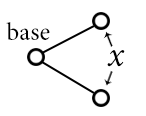
\includegraphics{literal-gadget.png}}
%\caption{The gadget for a literal. The two single-degree vertices represent a
%single literal, and are interpreted as true if they have the same color. The
%base vertex is always colored gray.}
%\label{fig:literal-gadget}
%\end{figure}

\begin{figure}
\floatbox[{\capbeside\thisfloatsetup{capbesideposition={right,top},capbesidewidth=10cm}}]{figure}[\FBwidth]
{\caption{The gadget for a literal. The two single-degree vertices represent a
single literal, and are interpreted as true if they have the same color. The
base vertex is always colored gray.}\label{fig:literal-gadget}}
{\scalebox{0.35}{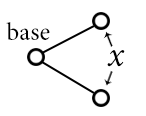
\includegraphics{literal-gadget.png}}}
\end{figure}


We connect two literal gadgets for $x, \overline{x}$ by a \emph{negation
gadget} in such a way that the gadget for $x$ is colored true if and only if
the gadget for $\overline{x}$ is colored false. The negation gadget is given in
Figure~\ref{fig:clause-and-negation-gadget}. In the diagram, the vertices
labeled 1 and 3 correspond to $x$, and those labeled 10 and 12 correspond to
$\overline{x}$. We start by showing that no proper coloring can exist if both
literal gadgets are colored true. If all four of these vertices are colored
white or all four are black, then vertices 6 and 7 must also have this color,
and so the coloring is not proper. If one pair is colored both white and the
other both black, then vertices 13 and 14 must be gray, and the coloring is
again not proper.  Next, we show that no proper coloring can exist if both
literal gadgets are colored false. First, if vertices 1 and 10 are white and
vertices 3 and 12 are black, then vertices 2 and 11 must be gray and the
coloring is not proper. If instead vertices 1 and 12 are white and vertices 3
and 10 black, then again vertices 13 and 14 must be gray. This covers all
possibilities up to symmetry.  It is also easy to see that whenever one literal
is colored true and the other false, one can extend it to a proper 3-coloring
of the whole gadget. 

\begin{figure}
\centering
\scalebox{0.35}{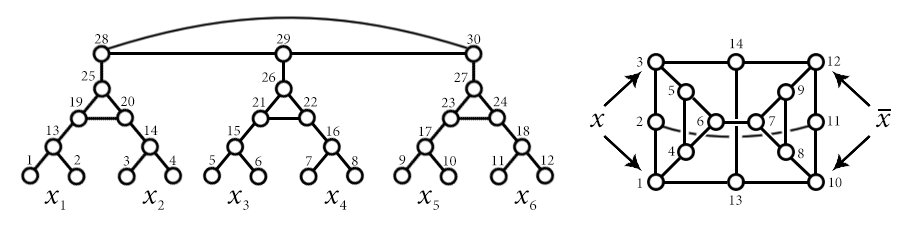
\includegraphics{clause-and-negation-gadget.png}}
\caption{Left: the gadget for a clause. Right: the negation gadget ensuring two
literals assume opposite truth values.} 
\label{fig:clause-and-negation-gadget}
\end{figure}


Now suppose we have a clause involving literals, without loss of generality
$x_1, \dots, x_6$. We construct the \emph{clause gadget} shown in
Figure~\ref{fig:clause-and-negation-gadget}, and claim that this gadget is
3-colorable if and only if at least one literal is colored true. Indeed, if the
literals are all colored false, then the vertices labeled 13 through 18 in the
diagram must be colored gray, and as a result the vertices 25, 26, 27
must be gray. This causes the central triangle to use only white and black,
and so it cannot be a proper coloring. On the other hand, if some literal is
colored true, we claim we can extend to a proper coloring of the whole gadget.
Suppose without loss of generality that the literal in question is $x_1$, and
that vertices 1 and 2 both are black. Then we see in
Figure~\ref{fig:clause-gadget-proof} how this extends to a proper coloring of
the entire gadget regardless of the truth assignments of the other literals (we
can always color their branches as if the literals were false). 

%\begin{figure}
%\centering
%\scalebox{0.35}{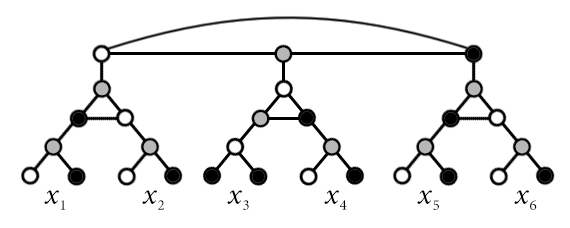
\includegraphics{clause-gadget-proof.png}}
%\caption{A valid coloring of the clause gadget when one variable (in this case $x_3$) is true.}
%\label{fig:clause-gadget-proof}
%\end{figure}

\begin{figure}
\floatbox[{\capbeside\thisfloatsetup{capbesideposition={left,center},capbesidewidth=5cm}}]{figure}[\FBwidth]
{\caption{A valid coloring of the clause gadget when one variable (in this case
$x_3$) is true.}\label{fig:clause-gadget-proof}}
{\scalebox{0.35}{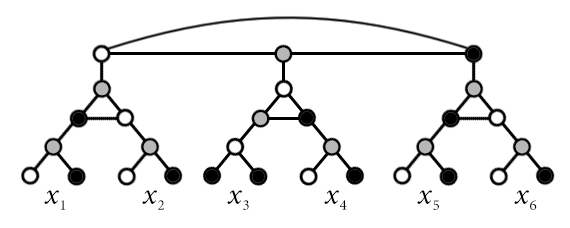
\includegraphics{clause-gadget-proof.png}}}
\end{figure}

It remains to show that $G$ is 1-resiliently 3-colorable when $\varphi$ is
1-resiliently satisfiable. This is because the worst that a new edge can do is
fix the truth assignment (perhaps indirectly) of at most one literal. Since the
original formula $\varphi$ is 1-resiliently satisfiable, $G$ maintains
3-colorability.  Additionally, the gadgets and the representation of truth were
chosen in such a way as to provide flexibility with respect to the chosen colors
for each vertex, so many edges will have no effect on the colorability of $G$. 

First, one can verify that the gadgets themselves are 1-resiliently
3-colorable.\footnote{These graphs are small enough to admit verification by
computer search.} We break down the analysis into eight cases based on the
endpoints of the added edge: within a single clause/negation/literal gadget,
between two distinct clause/negation/literal gadgets, between clause and
negation gadgets, and between negation and literal gadgets. We denote the added
edge by $e = (v,w)$ and call it \emph{good} if $G$ is still 3-colorable after
adding $e$. 

\emph{Literal Gadgets}. First, we argue that $e$ is good if it lies within or
across literal gadgets. Indeed, there is only one way to add an edge within a
literal gadget, and this has the effect of setting the literal to false. If $e$
lies across two gadgets then it has no effect: if $c$ is a proper coloring of
$G$ without $e$, then after adding $e$ either $c$ is still a proper coloring or
we can switch to a different representation of the truth value of $v$ or $w$ to
make $e$ properly colored (i.e. swap ``white white'' with ``black black,'' or
``white black'' with ``black white'' and recolor appropriately). 

\emph{Negation Gadgets}. Next we argue that $e$ is good if it involves a
negation gadget. Let $N$ be a negation gadget for the variable $x$. Indeed, by
1-resilience an edge within $N$ is good; $e$ only has a local effect within
negation gadgets, and it may result in fixing the truth value of $x$. Now
suppose $e$ has only one vertex $v$ in $N$. Figure~\ref{fig:coloring-negation}
shows two ways to color $N$, which together with reflections along the
horizontal axis of symmetry have the property that we may choose from at least
two colors for any vertex we wish. That is, if we are willing to fix the truth
value of $x$, then we may choose between one of two colors for $v$ so that $e$
is properly colored regardless of which color is adjacent to it.  

\begin{figure}
\centering
\scalebox{0.30}{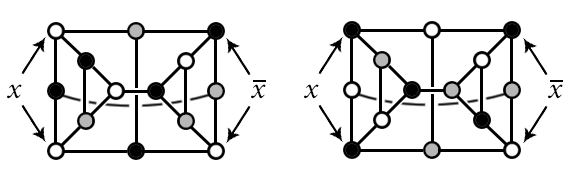
\includegraphics{coloring-negations.png}}
\caption{Two distinct ways to color a negation gadget without changing the
truth values of the literals. Only the rightmost center vertex cannot be given
a different color by a suitable switch between the two representations or a
reflection of the graph across the horizontal axis of symmetry. If the new edge
involves this vertex, we must fix the truth value appropriately.}
\label{fig:coloring-negation} \end{figure}

\emph{Clause Gadgets}. Suppose $e$ lies within a clause gadget or between two
clause gadgets. As with the negation gadget, it suffices to fix the truth value
of one variable suitably so that one may choose either of two colors for one
end of the new edge. Figure~\ref{fig:clause-clause-example} provides a detailed
illustration of one case. Here, we focus on two branches of two separate clause
gadgets, and add the new edge $e = (v,w)$. The added edge has the following
effect: if $x$ is false, then neither $y$ nor $z$ may be used to satisfy $C_2$
(as $w$ cannot be gray). This is no stronger than requiring that either $x$ be
true or $y$ and $z$ both be false, i.e., we add the clause $x \vee
(\overline{y} \wedge \overline{z})$ to $\varphi$. This clause can be
satisfied by fixing a single variable ($x$ to true), and $\varphi$ is
1-resilient, so we can still satisfy $\varphi$ and 3-color $G$.  The other cases
are analogous.

This proves that $G$ is 1-resilient when $\varphi$ is, and finishes the proof.
\end{proof}

Note the clause gadget in the proof comes from Kun~et~al.~\cite{KunPR13}.


%\begin{figure}
%\centering
%\scalebox{0.3}{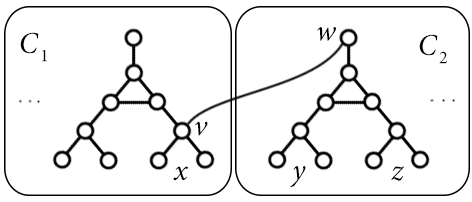
\includegraphics{clause-clause-example.png}}
%\caption{An example of an edge added between two clauses $C_1, C_2$.}
%\label{fig:clause-clause-example}
%\end{figure}

\begin{figure}
\floatbox[{\capbeside\thisfloatsetup{capbesideposition={right,center},capbesidewidth=4cm}}]{figure}[\FBwidth]
{\caption{An example of an edge added between two clauses $C_1,
C_2$.}\label{fig:clause-clause-example}}
{\scalebox{0.29}{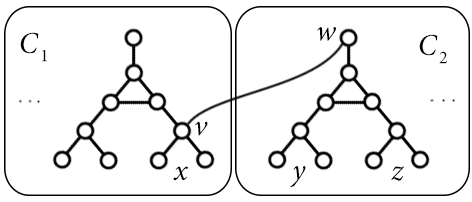
\includegraphics{clause-clause-example.png}}}
\end{figure}




\section{Discussion and open problems} \label{sec:open-problems}

The notion of resilience introduced in this paper leaves many questions
unanswered, both specific problems about graph coloring and more
general exploration of resilience in other combinatorial problems and CSPs. 

Regarding resilient graph coloring, our paper established the fact that
1-resilience doesn't affect the difficulty of graph coloring. However, the
question of 2-resilience is wide open, as is establishing linear lower bounds
without dependence on the 2-to-1 conjecture. There is also obvious room for
improvement in finding efficient algorithms for highly-resilient instances,
closing the gap between NP-hardness and tractability.

Additionally, we only scratched the surface of questions about resilient
satisfiability. For instance, while 3-resilient 3-SAT is vacuously trivial, it
is unclear whether 1- or 2-resilience is strong enough to make finding a
satisfying assignment of a 3-SAT instance easy. We conjecture that 1-resilience
is NP-hard and 2-resilience is tractable.

On the general side, there is a wealth of NP-complete problems that our
framework could be applied to, including Hamiltonian circuit, set cover,
3D-matching, 0-1 linear programming, and many others. Each presents its own
boundary between NP-hardness and tractability, and there are undoubtedly
interesting relationships across problems, as we showed with resilient
satisfiability and resilient coloring.

\subsection*{Acknowledgments}
We thank Shai Ben-David for helpful discussions.


\bibliographystyle{plain}
\bibliography{paper}


\end{document}
